\documentclass[1p]{elsarticle_modified}
%\bibliographystyle{elsarticle-num}

%\usepackage[colorlinks]{hyperref}
%\usepackage{abbrmath_seonhwa} %\Abb, \Ascr, \Acal ,\Abf, \Afrak
\usepackage{amsfonts}
\usepackage{amssymb}
\usepackage{amsmath}
\usepackage{amsthm}
\usepackage{scalefnt}
\usepackage{amsbsy}
\usepackage{kotex}
\usepackage{caption}
\usepackage{subfig}
\usepackage{color}
\usepackage{graphicx}
\usepackage{xcolor} %% white, black, red, green, blue, cyan, magenta, yellow
\usepackage{float}
\usepackage{setspace}
\usepackage{hyperref}

\usepackage{tikz}
\usetikzlibrary{arrows}

\usepackage{multirow}
\usepackage{array} % fixed length table
\usepackage{hhline}

%%%%%%%%%%%%%%%%%%%%%
\makeatletter
\renewcommand*\env@matrix[1][\arraystretch]{%
	\edef\arraystretch{#1}%
	\hskip -\arraycolsep
	\let\@ifnextchar\new@ifnextchar
	\array{*\c@MaxMatrixCols c}}
\makeatother %https://tex.stackexchange.com/questions/14071/how-can-i-increase-the-line-spacing-in-a-matrix
%%%%%%%%%%%%%%%

\usepackage[normalem]{ulem}

\newcommand{\msout}[1]{\ifmmode\text{\sout{\ensuremath{#1}}}\else\sout{#1}\fi}
%SOURCE: \msout is \stkout macro in https://tex.stackexchange.com/questions/20609/strikeout-in-math-mode

\newcommand{\cancel}[1]{
	\ifmmode
	{\color{red}\msout{#1}}
	\else
	{\color{red}\sout{#1}}
	\fi
}

\newcommand{\add}[1]{
	{\color{blue}\uwave{#1}}
}

\newcommand{\replace}[2]{
	\ifmmode
	{\color{red}\msout{#1}}{\color{blue}\uwave{#2}}
	\else
	{\color{red}\sout{#1}}{\color{blue}\uwave{#2}}
	\fi
}

\newcommand{\Sol}{\mathcal{S}} %segment
\newcommand{\D}{D} %diagram
\newcommand{\A}{\mathcal{A}} %arc


%%%%%%%%%%%%%%%%%%%%%%%%%%%%%5 test

\def\sl{\operatorname{\textup{SL}}(2,\Cbb)}
\def\psl{\operatorname{\textup{PSL}}(2,\Cbb)}
\def\quan{\mkern 1mu \triangleright \mkern 1mu}

\theoremstyle{definition}
\newtheorem{thm}{Theorem}[section]
\newtheorem{prop}[thm]{Proposition}
\newtheorem{lem}[thm]{Lemma}
\newtheorem{ques}[thm]{Question}
\newtheorem{cor}[thm]{Corollary}
\newtheorem{defn}[thm]{Definition}
\newtheorem{exam}[thm]{Example}
\newtheorem{rmk}[thm]{Remark}
\newtheorem{alg}[thm]{Algorithm}

\newcommand{\I}{\sqrt{-1}}
\begin{document}

%\begin{frontmatter}
%
%\title{Boundary parabolic representations of knots up to 8 crossings}
%
%%% Group authors per affiliation:
%\author{Yunhi Cho} 
%\address{Department of Mathematics, University of Seoul, Seoul, Korea}
%\ead{yhcho@uos.ac.kr}
%
%
%\author{Seonhwa Kim} %\fnref{s_kim}}
%\address{Center for Geometry and Physics, Institute for Basic Science, Pohang, 37673, Korea}
%\ead{ryeona17@ibs.re.kr}
%
%\author{Hyuk Kim}
%\address{Department of Mathematical Sciences, Seoul National University, Seoul 08826, Korea}
%\ead{hyukkim@snu.ac.kr}
%
%\author{Seokbeom Yoon}
%\address{Department of Mathematical Sciences, Seoul National University, Seoul, 08826,  Korea}
%\ead{sbyoon15@snu.ac.kr}
%
%\begin{abstract}
%We find all boundary parabolic representation of knots up to 8 crossings.
%
%\end{abstract}
%\begin{keyword}
%    \MSC[2010] 57M25 
%\end{keyword}
%
%\end{frontmatter}

%\linenumbers
%\tableofcontents
%
\newcommand\colored[1]{\textcolor{white}{\rule[-0.35ex]{0.8em}{1.4ex}}\kern-0.8em\color{red} #1}%
%\newcommand\colored[1]{\textcolor{white}{ #1}\kern-2.17ex	\textcolor{white}{ #1}\kern-1.81ex	\textcolor{white}{ #1}\kern-2.15ex\color{red}#1	}

{\Large $\underline{11a_{325}~(K11a_{325})}$}

\setlength{\tabcolsep}{10pt}
\renewcommand{\arraystretch}{1.6}
\vspace{1cm}\begin{tabular}{m{100pt}>{\centering\arraybackslash}m{274pt}}
\multirow{5}{120pt}{
	\centering
	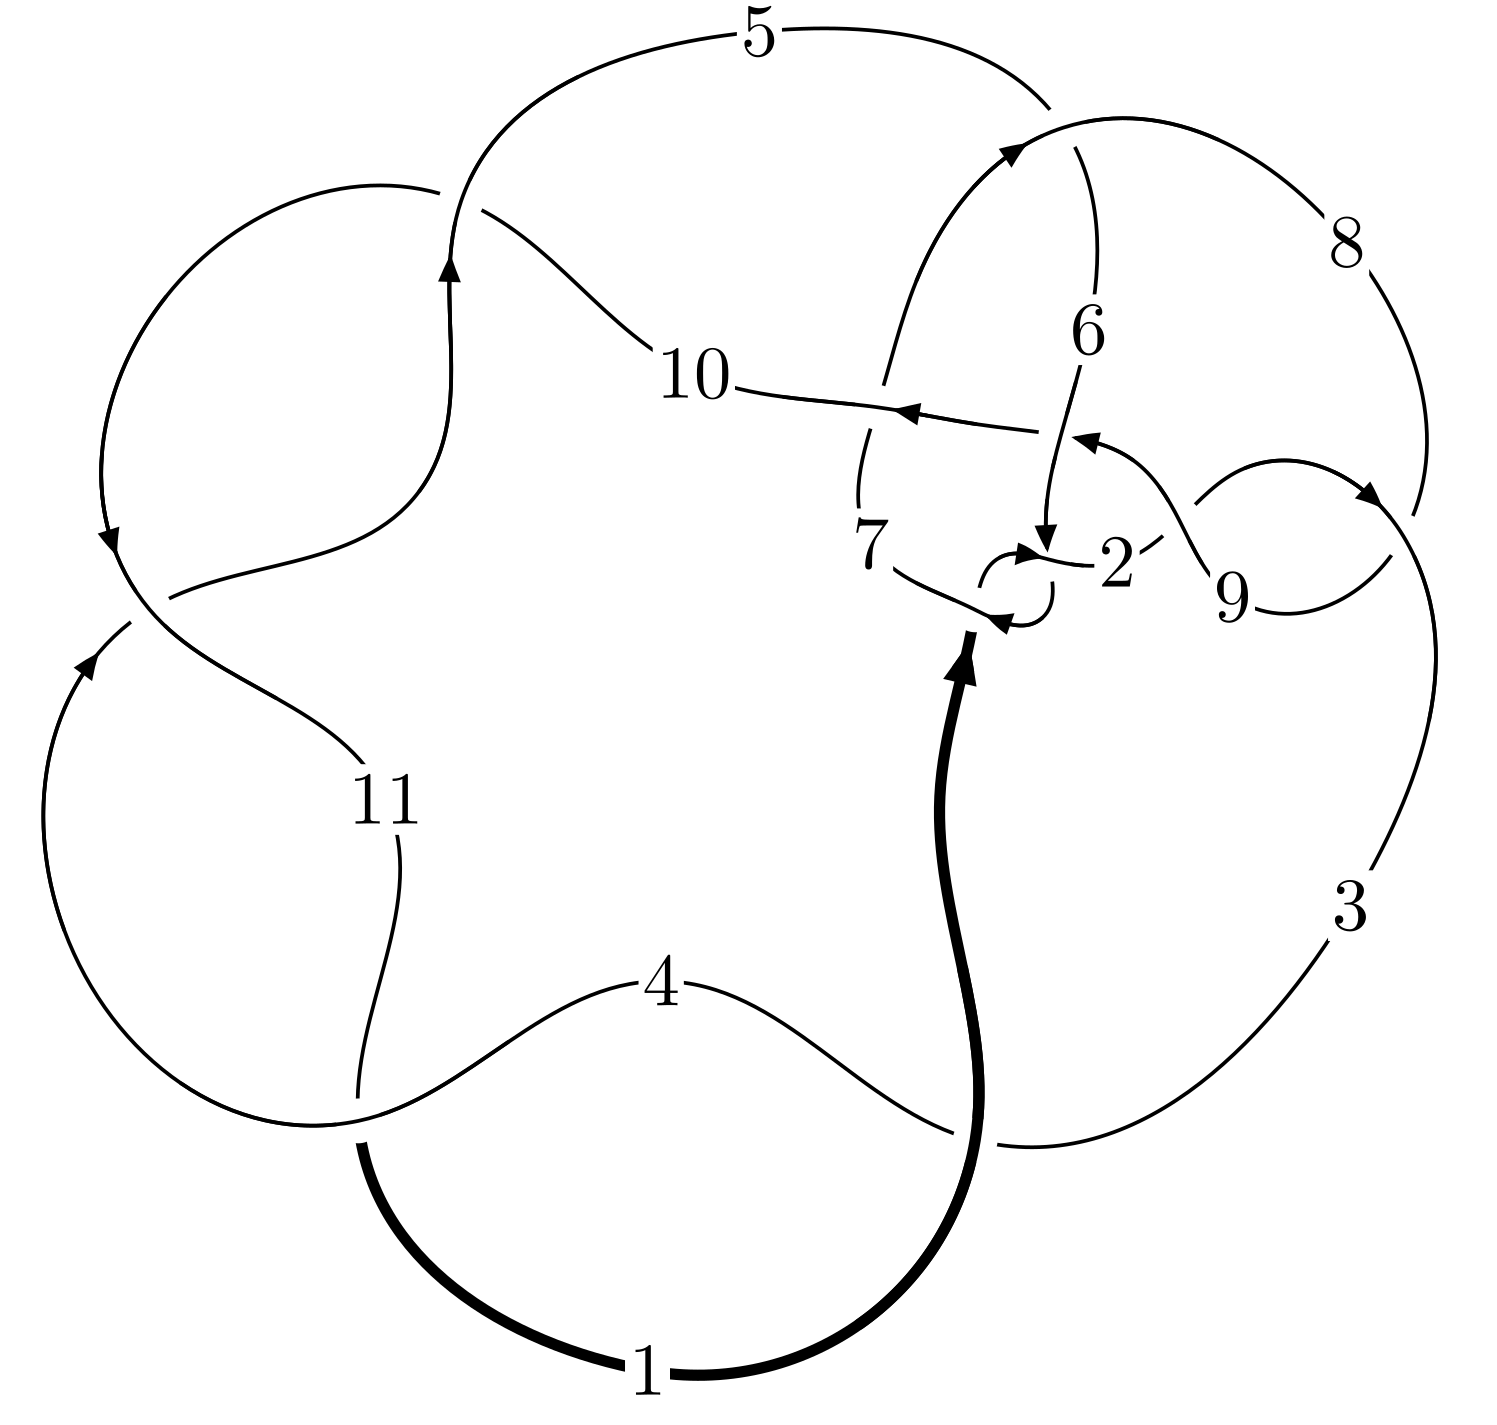
\includegraphics[width=112pt]{../../../GIT/diagram.site/Diagrams/png/574_11a_325.png}\\
\ \ \ A knot diagram\footnotemark}&
\allowdisplaybreaks
\textbf{Linearized knot diagam} \\
\cline{2-2}
 &
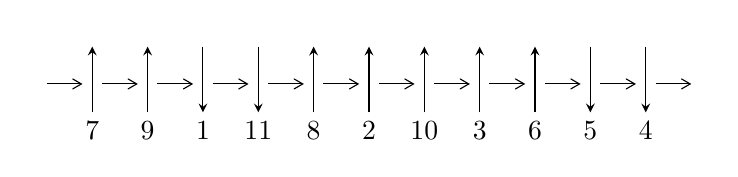
\begin{tikzpicture}[x=20pt, y=17pt]
	% nodes
	\node (C0) at (0, 0) {};
	\node (C1) at (1, 0) {};
	\node (C1U) at (1, +1) {};
	\node (C1D) at (1, -1) {7};

	\node (C2) at (2, 0) {};
	\node (C2U) at (2, +1) {};
	\node (C2D) at (2, -1) {9};

	\node (C3) at (3, 0) {};
	\node (C3U) at (3, +1) {};
	\node (C3D) at (3, -1) {1};

	\node (C4) at (4, 0) {};
	\node (C4U) at (4, +1) {};
	\node (C4D) at (4, -1) {11};

	\node (C5) at (5, 0) {};
	\node (C5U) at (5, +1) {};
	\node (C5D) at (5, -1) {8};

	\node (C6) at (6, 0) {};
	\node (C6U) at (6, +1) {};
	\node (C6D) at (6, -1) {2};

	\node (C7) at (7, 0) {};
	\node (C7U) at (7, +1) {};
	\node (C7D) at (7, -1) {10};

	\node (C8) at (8, 0) {};
	\node (C8U) at (8, +1) {};
	\node (C8D) at (8, -1) {3};

	\node (C9) at (9, 0) {};
	\node (C9U) at (9, +1) {};
	\node (C9D) at (9, -1) {6};

	\node (C10) at (10, 0) {};
	\node (C10U) at (10, +1) {};
	\node (C10D) at (10, -1) {5};

	\node (C11) at (11, 0) {};
	\node (C11U) at (11, +1) {};
	\node (C11D) at (11, -1) {4};
	\node (C12) at (12, 0) {};

	% arrows
	\draw[->,>={angle 60}]
	(C0) edge (C1) (C1) edge (C2) (C2) edge (C3) (C3) edge (C4) (C4) edge (C5) (C5) edge (C6) (C6) edge (C7) (C7) edge (C8) (C8) edge (C9) (C9) edge (C10) (C10) edge (C11) (C11) edge (C12) ;	\draw[->,>=stealth]
	(C1D) edge (C1U) (C2D) edge (C2U) (C3U) edge (C3D) (C4U) edge (C4D) (C5D) edge (C5U) (C6D) edge (C6U) (C7D) edge (C7U) (C8D) edge (C8U) (C9D) edge (C9U) (C10U) edge (C10D) (C11U) edge (C11D) ;
	\end{tikzpicture} \\
\hhline{~~} \\& 
\textbf{Solving Sequence} \\ \cline{2-2} 
 &
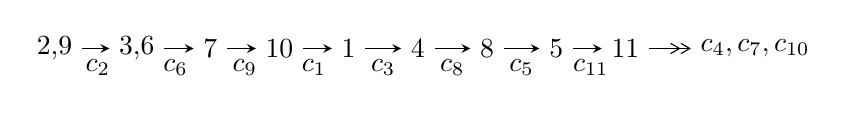
\begin{tikzpicture}[x=25pt, y=7pt]
	% node
	\node (A0) at (-1/8, 0) {2,9};
	\node (A1) at (17/16, 0) {3,6};
	\node (A2) at (17/8, 0) {7};
	\node (A3) at (25/8, 0) {10};
	\node (A4) at (33/8, 0) {1};
	\node (A5) at (41/8, 0) {4};
	\node (A6) at (49/8, 0) {8};
	\node (A7) at (57/8, 0) {5};
	\node (A8) at (65/8, 0) {11};
	\node (C1) at (1/2, -1) {$c_{2}$};
	\node (C2) at (13/8, -1) {$c_{6}$};
	\node (C3) at (21/8, -1) {$c_{9}$};
	\node (C4) at (29/8, -1) {$c_{1}$};
	\node (C5) at (37/8, -1) {$c_{3}$};
	\node (C6) at (45/8, -1) {$c_{8}$};
	\node (C7) at (53/8, -1) {$c_{5}$};
	\node (C8) at (61/8, -1) {$c_{11}$};
	\node (A9) at (10, 0) {$c_{4},c_{7},c_{10}$};

	% edge
	\draw[->,>=stealth]	
	(A0) edge (A1) (A1) edge (A2) (A2) edge (A3) (A3) edge (A4) (A4) edge (A5) (A5) edge (A6) (A6) edge (A7) (A7) edge (A8) ;
	\draw[->>,>={angle 60}]	
	(A8) edge (A9);
\end{tikzpicture} \\ 

\end{tabular} \\

\footnotetext{
The image of knot diagram is generated by the software ``\textbf{Draw programme}" developed by Andrew Bartholomew(\url{http://www.layer8.co.uk/maths/draw/index.htm\#Running-draw}), where we modified some parts for our purpose(\url{https://github.com/CATsTAILs/LinksPainter}).
}\phantom \\ \newline 
\centering \textbf{Ideals for irreducible components\footnotemark of $X_{\text{par}}$} 
 
\begin{align*}
I^u_{1}&=\langle 
b- u,\;-36589 u^{20}-75173 u^{19}+\cdots+133419 a+168070,\;u^{21}+7 u^{19}+\cdots+2 u-1\rangle \\
I^u_{2}&=\langle 
-1.50267\times10^{47} u^{35}+7.89794\times10^{47} u^{34}+\cdots+8.17083\times10^{48} b+1.26464\times10^{50},\\
\phantom{I^u_{2}}&\phantom{= \langle  }1.51725\times10^{32} u^{35}+1.19597\times10^{32} u^{34}+\cdots+1.00338\times10^{33} a-5.77606\times10^{33},\;u^{36}+u^{35}+\cdots-88 u+121\rangle \\
I^u_{3}&=\langle 
b+u,\;- u^9- u^8-5 u^7-5 u^6-11 u^5-9 u^4-11 u^3-6 u^2+a-5 u-1,\\
\phantom{I^u_{3}}&\phantom{= \langle  }u^{10}+5 u^8+u^7+10 u^6+3 u^5+9 u^4+3 u^3+4 u^2+1\rangle \\
\\
\end{align*}
\raggedright * 3 irreducible components of $\dim_{\mathbb{C}}=0$, with total 67 representations.\\
\footnotetext{All coefficients of polynomials are rational numbers. But the coefficients are sometimes approximated in decimal forms when there is not enough margin.}
\newpage
\renewcommand{\arraystretch}{1}
\centering \section*{I. $I^u_{1}= \langle b- u,\;-3.66\times10^{4} u^{20}-7.52\times10^{4} u^{19}+\cdots+1.33\times10^{5} a+1.68\times10^{5},\;u^{21}+7 u^{19}+\cdots+2 u-1 \rangle$}
\flushleft \textbf{(i) Arc colorings}\\
\begin{tabular}{m{7pt} m{180pt} m{7pt} m{180pt} }
\flushright $a_{2}=$&$\begin{pmatrix}1\\0\end{pmatrix}$ \\
\flushright $a_{9}=$&$\begin{pmatrix}0\\u\end{pmatrix}$ \\
\flushright $a_{3}=$&$\begin{pmatrix}1\\- u^2\end{pmatrix}$ \\
\flushright $a_{6}=$&$\begin{pmatrix}0.274241 u^{20}+0.563435 u^{19}+\cdots-0.725182 u-1.25972\\u\end{pmatrix}$ \\
\flushright $a_{7}=$&$\begin{pmatrix}0.274241 u^{20}+0.563435 u^{19}+\cdots+0.274818 u-1.25972\\u\end{pmatrix}$ \\
\flushright $a_{10}=$&$\begin{pmatrix}-0.364446 u^{20}-0.326445 u^{19}+\cdots+0.141996 u+0.459290\\-0.171242 u^{20}-0.393302 u^{19}+\cdots+0.147370 u+0.563435\end{pmatrix}$ \\
\flushright $a_{1}=$&$\begin{pmatrix}0.563435 u^{20}-0.171242 u^{19}+\cdots-1.80820 u+1.27424\\u^2\end{pmatrix}$ \\
\flushright $a_{4}=$&$\begin{pmatrix}-0.535284 u^{20}+0.170748 u^{19}+\cdots+1.53655 u+0.520353\\0.0475045 u^{20}+0.315750 u^{19}+\cdots+0.00530659 u-0.199304\end{pmatrix}$ \\
\flushright $a_{8}=$&$\begin{pmatrix}- u\\u^3+u\end{pmatrix}$ \\
\flushright $a_{5}=$&$\begin{pmatrix}0.644788 u^{20}+0.909233 u^{19}+\cdots-0.487914 u-1.42985\\-0.254102 u^{20}+0.0146306 u^{19}+\cdots+1.08378 u-0.175665\end{pmatrix}$ \\
\flushright $a_{11}=$&$\begin{pmatrix}-0.582496 u^{20}-0.577624 u^{19}+\cdots-0.376093 u+0.851783\\-0.441159 u^{20}-0.406276 u^{19}+\cdots+0.464934 u+0.246457\end{pmatrix}$\\ \flushright $a_{11}=$&$\begin{pmatrix}-0.582496 u^{20}-0.577624 u^{19}+\cdots-0.376093 u+0.851783\\-0.441159 u^{20}-0.406276 u^{19}+\cdots+0.464934 u+0.246457\end{pmatrix}$\\&\end{tabular}
\flushleft \textbf{(ii) Obstruction class $= -1$}\\~\\
\flushleft \textbf{(iii) Cusp Shapes $= \frac{129645}{44473} u^{20}+\frac{33237}{44473} u^{19}+\cdots-\frac{265846}{44473} u+\frac{357015}{44473}$}\\~\\
\newpage\renewcommand{\arraystretch}{1}
\flushleft \textbf{(iv) u-Polynomials at the component}\newline \\
\begin{tabular}{m{50pt}|m{274pt}}
Crossings & \hspace{64pt}u-Polynomials at each crossing \\
\hline $$\begin{aligned}c_{1},c_{2},c_{6}\\c_{8}\end{aligned}$$&$\begin{aligned}
&u^{21}+7 u^{19}+\cdots+2 u-1
\end{aligned}$\\
\hline $$\begin{aligned}c_{3},c_{4},c_{10}\\c_{11}\end{aligned}$$&$\begin{aligned}
&u^{21}-6 u^{20}+\cdots+38 u-4
\end{aligned}$\\
\hline $$\begin{aligned}c_{5},c_{7}\end{aligned}$$&$\begin{aligned}
&u^{21}-6 u^{19}+\cdots-7 u-1
\end{aligned}$\\
\hline $$\begin{aligned}c_{9}\end{aligned}$$&$\begin{aligned}
&u^{21}-18 u^{20}+\cdots+4352 u-512
\end{aligned}$\\
\hline
\end{tabular}\\~\\
\newpage\renewcommand{\arraystretch}{1}
\flushleft \textbf{(v) Riley Polynomials at the component}\newline \\
\begin{tabular}{m{50pt}|m{274pt}}
Crossings & \hspace{64pt}Riley Polynomials at each crossing \\
\hline $$\begin{aligned}c_{1},c_{2},c_{6}\\c_{8}\end{aligned}$$&$\begin{aligned}
&y^{21}+14 y^{20}+\cdots+12 y^2-1
\end{aligned}$\\
\hline $$\begin{aligned}c_{3},c_{4},c_{10}\\c_{11}\end{aligned}$$&$\begin{aligned}
&y^{21}+24 y^{20}+\cdots+108 y-16
\end{aligned}$\\
\hline $$\begin{aligned}c_{5},c_{7}\end{aligned}$$&$\begin{aligned}
&y^{21}-12 y^{20}+\cdots+27 y-1
\end{aligned}$\\
\hline $$\begin{aligned}c_{9}\end{aligned}$$&$\begin{aligned}
&y^{21}+2 y^{20}+\cdots+65536 y-262144
\end{aligned}$\\
\hline
\end{tabular}\\~\\
\newpage\flushleft \textbf{(vi) Complex Volumes and Cusp Shapes}
$$\begin{array}{c|c|c}  
\text{Solutions to }I^u_{1}& \I (\text{vol} + \sqrt{-1}CS) & \text{Cusp shape}\\
 \hline 
\begin{aligned}
u &= -0.089530 + 0.984696 I \\
a &= -0.10595 + 1.89249 I \\
b &= -0.089530 + 0.984696 I\end{aligned}
 & -0.41138 - 2.40421 I & \phantom{-}1.72315 + 4.22426 I \\ \hline\begin{aligned}
u &= -0.089530 - 0.984696 I \\
a &= -0.10595 - 1.89249 I \\
b &= -0.089530 - 0.984696 I\end{aligned}
 & -0.41138 + 2.40421 I & \phantom{-}1.72315 - 4.22426 I \\ \hline\begin{aligned}
u &= -0.709348 + 0.727206 I \\
a &= \phantom{-}1.013410 - 0.479147 I \\
b &= -0.709348 + 0.727206 I\end{aligned}
 & \phantom{-}8.83155 - 2.25669 I & \phantom{-}7.66847 + 3.47538 I \\ \hline\begin{aligned}
u &= -0.709348 - 0.727206 I \\
a &= \phantom{-}1.013410 + 0.479147 I \\
b &= -0.709348 - 0.727206 I\end{aligned}
 & \phantom{-}8.83155 + 2.25669 I & \phantom{-}7.66847 - 3.47538 I \\ \hline\begin{aligned}
u &= \phantom{-}0.241671 + 1.064200 I \\
a &= \phantom{-}0.20712 + 1.60998 I \\
b &= \phantom{-}0.241671 + 1.064200 I\end{aligned}
 & \phantom{-}6.84048 + 5.76907 I & \phantom{-}4.07518 - 4.56239 I \\ \hline\begin{aligned}
u &= \phantom{-}0.241671 - 1.064200 I \\
a &= \phantom{-}0.20712 - 1.60998 I \\
b &= \phantom{-}0.241671 - 1.064200 I\end{aligned}
 & \phantom{-}6.84048 - 5.76907 I & \phantom{-}4.07518 + 4.56239 I \\ \hline\begin{aligned}
u &= \phantom{-}0.819786 + 0.389956 I \\
a &= -0.690629 + 0.984448 I \\
b &= \phantom{-}0.819786 + 0.389956 I\end{aligned}
 & \phantom{-}10.89630 - 2.89300 I & \phantom{-}9.55027 + 0.75508 I \\ \hline\begin{aligned}
u &= \phantom{-}0.819786 - 0.389956 I \\
a &= -0.690629 - 0.984448 I \\
b &= \phantom{-}0.819786 - 0.389956 I\end{aligned}
 & \phantom{-}10.89630 + 2.89300 I & \phantom{-}9.55027 - 0.75508 I \\ \hline\begin{aligned}
u &= \phantom{-}0.420437 + 1.104620 I \\
a &= -1.57981 - 0.05796 I \\
b &= \phantom{-}0.420437 + 1.104620 I\end{aligned}
 & -1.62807 + 2.56050 I & \phantom{-}4.45468 - 5.57761 I \\ \hline\begin{aligned}
u &= \phantom{-}0.420437 - 1.104620 I \\
a &= -1.57981 + 0.05796 I \\
b &= \phantom{-}0.420437 - 1.104620 I\end{aligned}
 & -1.62807 - 2.56050 I & \phantom{-}4.45468 + 5.57761 I\\
 \hline 
 \end{array}$$\newpage$$\begin{array}{c|c|c}  
\text{Solutions to }I^u_{1}& \I (\text{vol} + \sqrt{-1}CS) & \text{Cusp shape}\\
 \hline 
\begin{aligned}
u &= -0.628080 + 0.259561 I \\
a &= \phantom{-}0.99006 + 1.03585 I \\
b &= -0.628080 + 0.259561 I\end{aligned}
 & \phantom{-}2.86823 + 1.78605 I & \phantom{-}10.67672 - 1.49019 I \\ \hline\begin{aligned}
u &= -0.628080 - 0.259561 I \\
a &= \phantom{-}0.99006 - 1.03585 I \\
b &= -0.628080 - 0.259561 I\end{aligned}
 & \phantom{-}2.86823 - 1.78605 I & \phantom{-}10.67672 + 1.49019 I \\ \hline\begin{aligned}
u &= -0.476681 + 1.277180 I \\
a &= \phantom{-}1.297630 + 0.183037 I \\
b &= -0.476681 + 1.277180 I\end{aligned}
 & -5.88506 - 6.78578 I & -0.85150 + 5.15843 I \\ \hline\begin{aligned}
u &= -0.476681 - 1.277180 I \\
a &= \phantom{-}1.297630 - 0.183037 I \\
b &= -0.476681 - 1.277180 I\end{aligned}
 & -5.88506 + 6.78578 I & -0.85150 - 5.15843 I \\ \hline\begin{aligned}
u &= \phantom{-}0.274697 + 0.539680 I \\
a &= -0.715108 - 0.945305 I \\
b &= \phantom{-}0.274697 + 0.539680 I\end{aligned}
 & \phantom{-}0.19501 + 1.45011 I & \phantom{-}2.94900 - 3.15728 I \\ \hline\begin{aligned}
u &= \phantom{-}0.274697 - 0.539680 I \\
a &= -0.715108 + 0.945305 I \\
b &= \phantom{-}0.274697 - 0.539680 I\end{aligned}
 & \phantom{-}0.19501 - 1.45011 I & \phantom{-}2.94900 + 3.15728 I \\ \hline\begin{aligned}
u &= \phantom{-}0.55258 + 1.36736 I \\
a &= -1.134920 + 0.188406 I \\
b &= \phantom{-}0.55258 + 1.36736 I\end{aligned}
 & -4.07842 + 11.41590 I & \phantom{-}1.76912 - 8.47188 I \\ \hline\begin{aligned}
u &= \phantom{-}0.55258 - 1.36736 I \\
a &= -1.134920 - 0.188406 I \\
b &= \phantom{-}0.55258 - 1.36736 I\end{aligned}
 & -4.07842 - 11.41590 I & \phantom{-}1.76912 + 8.47188 I \\ \hline\begin{aligned}
u &= -0.62291 + 1.42854 I \\
a &= \phantom{-}1.038290 + 0.171241 I \\
b &= -0.62291 + 1.42854 I\end{aligned}
 & \phantom{-}4.0861 - 14.4126 I & \phantom{-}4.28661 + 7.20471 I \\ \hline\begin{aligned}
u &= -0.62291 - 1.42854 I \\
a &= \phantom{-}1.038290 - 0.171241 I \\
b &= -0.62291 - 1.42854 I\end{aligned}
 & \phantom{-}4.0861 + 14.4126 I & \phantom{-}4.28661 - 7.20471 I\\
 \hline 
 \end{array}$$\newpage$$\begin{array}{c|c|c}  
\text{Solutions to }I^u_{1}& \I (\text{vol} + \sqrt{-1}CS) & \text{Cusp shape}\\
 \hline 
\begin{aligned}
u &= \phantom{-}0.434772\phantom{ +0.000000I} \\
a &= -1.64018\phantom{ +0.000000I} \\
b &= \phantom{-}0.434772\phantom{ +0.000000I}\end{aligned}
 & \phantom{-}0.983801\phantom{ +0.000000I} & \phantom{-}10.3970\phantom{ +0.000000I}\\
 \hline 
 \end{array}$$\newpage\newpage\renewcommand{\arraystretch}{1}
\centering \section*{II. $I^u_{2}= \langle -1.50\times10^{47} u^{35}+7.90\times10^{47} u^{34}+\cdots+8.17\times10^{48} b+1.26\times10^{50},\;1.52\times10^{32} u^{35}+1.20\times10^{32} u^{34}+\cdots+1.00\times10^{33} a-5.78\times10^{33},\;u^{36}+u^{35}+\cdots-88 u+121 \rangle$}
\flushleft \textbf{(i) Arc colorings}\\
\begin{tabular}{m{7pt} m{180pt} m{7pt} m{180pt} }
\flushright $a_{2}=$&$\begin{pmatrix}1\\0\end{pmatrix}$ \\
\flushright $a_{9}=$&$\begin{pmatrix}0\\u\end{pmatrix}$ \\
\flushright $a_{3}=$&$\begin{pmatrix}1\\- u^2\end{pmatrix}$ \\
\flushright $a_{6}=$&$\begin{pmatrix}-0.151215 u^{35}-0.119194 u^{34}+\cdots-29.7352 u+5.75661\\0.0183906 u^{35}-0.0966602 u^{34}+\cdots+19.1446 u-15.4775\end{pmatrix}$ \\
\flushright $a_{7}=$&$\begin{pmatrix}-0.132824 u^{35}-0.215854 u^{34}+\cdots-10.5906 u-9.72088\\0.0183906 u^{35}-0.0966602 u^{34}+\cdots+19.1446 u-15.4775\end{pmatrix}$ \\
\flushright $a_{10}=$&$\begin{pmatrix}-0.142950 u^{35}-0.110929 u^{34}+\cdots-23.0740 u+5.02934\\-0.0996243 u^{35}-0.0572367 u^{34}+\cdots-8.34916 u+0.642617\end{pmatrix}$ \\
\flushright $a_{1}=$&$\begin{pmatrix}0.235158 u^{35}+0.150714 u^{34}+\cdots+43.1286 u-10.6737\\0.240469 u^{35}+0.255649 u^{34}+\cdots+27.1442 u-2.79189\end{pmatrix}$ \\
\flushright $a_{4}=$&$\begin{pmatrix}-0.231245 u^{35}-0.605373 u^{34}+\cdots+13.5883 u-48.7866\\-0.0590880 u^{35}-0.422425 u^{34}+\cdots+36.6423 u-48.0768\end{pmatrix}$ \\
\flushright $a_{8}=$&$\begin{pmatrix}- u\\u^3+u\end{pmatrix}$ \\
\flushright $a_{5}=$&$\begin{pmatrix}-0.181447 u^{35}-0.279824 u^{34}+\cdots-22.4844 u-9.51522\\0.0242422 u^{35}-0.0920959 u^{34}+\cdots+19.7108 u-15.9838\end{pmatrix}$ \\
\flushright $a_{11}=$&$\begin{pmatrix}-0.342315 u^{35}-0.0676417 u^{34}+\cdots-73.5185 u+27.0801\\-0.340322 u^{35}-0.200761 u^{34}+\cdots-48.3147 u+13.7797\end{pmatrix}$\\ \flushright $a_{11}=$&$\begin{pmatrix}-0.342315 u^{35}-0.0676417 u^{34}+\cdots-73.5185 u+27.0801\\-0.340322 u^{35}-0.200761 u^{34}+\cdots-48.3147 u+13.7797\end{pmatrix}$\\&\end{tabular}
\flushleft \textbf{(ii) Obstruction class $= -1$}\\~\\
\flushleft \textbf{(iii) Cusp Shapes $= -0.0198670 u^{35}+0.230113 u^{34}+\cdots-18.4708 u+28.1644$}\\~\\
\newpage\renewcommand{\arraystretch}{1}
\flushleft \textbf{(iv) u-Polynomials at the component}\newline \\
\begin{tabular}{m{50pt}|m{274pt}}
Crossings & \hspace{64pt}u-Polynomials at each crossing \\
\hline $$\begin{aligned}c_{1},c_{2},c_{6}\\c_{8}\end{aligned}$$&$\begin{aligned}
&u^{36}+u^{35}+\cdots-88 u+121
\end{aligned}$\\
\hline $$\begin{aligned}c_{3},c_{4},c_{10}\\c_{11}\end{aligned}$$&$\begin{aligned}
&(u^9+u^8+6 u^7+5 u^6+11 u^5+7 u^4+6 u^3+2 u^2+u+1)^4
\end{aligned}$\\
\hline $$\begin{aligned}c_{5},c_{7}\end{aligned}$$&$\begin{aligned}
&u^{36}+9 u^{35}+\cdots-8 u+1
\end{aligned}$\\
\hline $$\begin{aligned}c_{9}\end{aligned}$$&$\begin{aligned}
&(u^2+u+1)^{18}
\end{aligned}$\\
\hline
\end{tabular}\\~\\
\newpage\renewcommand{\arraystretch}{1}
\flushleft \textbf{(v) Riley Polynomials at the component}\newline \\
\begin{tabular}{m{50pt}|m{274pt}}
Crossings & \hspace{64pt}Riley Polynomials at each crossing \\
\hline $$\begin{aligned}c_{1},c_{2},c_{6}\\c_{8}\end{aligned}$$&$\begin{aligned}
&y^{36}+27 y^{35}+\cdots+187308 y+14641
\end{aligned}$\\
\hline $$\begin{aligned}c_{3},c_{4},c_{10}\\c_{11}\end{aligned}$$&$\begin{aligned}
&(y^9+11 y^8+48 y^7+105 y^6+121 y^5+73 y^4+20 y^3-6 y^2-3 y-1)^4
\end{aligned}$\\
\hline $$\begin{aligned}c_{5},c_{7}\end{aligned}$$&$\begin{aligned}
&y^{36}+3 y^{35}+\cdots-44 y+1
\end{aligned}$\\
\hline $$\begin{aligned}c_{9}\end{aligned}$$&$\begin{aligned}
&(y^2+y+1)^{18}
\end{aligned}$\\
\hline
\end{tabular}\\~\\
\newpage\flushleft \textbf{(vi) Complex Volumes and Cusp Shapes}
$$\begin{array}{c|c|c}  
\text{Solutions to }I^u_{2}& \I (\text{vol} + \sqrt{-1}CS) & \text{Cusp shape}\\
 \hline 
\begin{aligned}
u &= -0.039626 + 0.981491 I \\
a &= \phantom{-}0.860387 - 0.544166 I \\
b &= -0.29688 - 1.73262 I\end{aligned}
 & \phantom{-}2.12882 - 0.18400 I & \phantom{-}2.24115 - 0.41812 I \\ \hline\begin{aligned}
u &= -0.039626 - 0.981491 I \\
a &= \phantom{-}0.860387 + 0.544166 I \\
b &= -0.29688 + 1.73262 I\end{aligned}
 & \phantom{-}2.12882 + 0.18400 I & \phantom{-}2.24115 + 0.41812 I \\ \hline\begin{aligned}
u &= \phantom{-}0.154191 + 1.093140 I \\
a &= \phantom{-}0.840038 - 0.338907 I \\
b &= -0.794470 + 0.015853 I\end{aligned}
 & -2.09801 + 2.02988 I & -0.33330 - 3.46410 I \\ \hline\begin{aligned}
u &= \phantom{-}0.154191 - 1.093140 I \\
a &= \phantom{-}0.840038 + 0.338907 I \\
b &= -0.794470 - 0.015853 I\end{aligned}
 & -2.09801 - 2.02988 I & -0.33330 + 3.46410 I \\ \hline\begin{aligned}
u &= -0.129901 + 1.110370 I \\
a &= -0.821381 - 0.354208 I \\
b &= \phantom{-}0.40998 - 1.53870 I\end{aligned}
 & -4.89942 - 0.92019 I & -1.44626 - 2.77537 I \\ \hline\begin{aligned}
u &= -0.129901 - 1.110370 I \\
a &= -0.821381 + 0.354208 I \\
b &= \phantom{-}0.40998 + 1.53870 I\end{aligned}
 & -4.89942 + 0.92019 I & -1.44626 + 2.77537 I \\ \hline\begin{aligned}
u &= \phantom{-}1.165700 + 0.010466 I \\
a &= \phantom{-}0.435562 + 0.739012 I \\
b &= -0.334918 - 1.124560 I\end{aligned}
 & \phantom{-}0.22800 + 5.44061 I & \phantom{-}3.88238 - 7.86053 I \\ \hline\begin{aligned}
u &= \phantom{-}1.165700 - 0.010466 I \\
a &= \phantom{-}0.435562 - 0.739012 I \\
b &= -0.334918 + 1.124560 I\end{aligned}
 & \phantom{-}0.22800 - 5.44061 I & \phantom{-}3.88238 + 7.86053 I \\ \hline\begin{aligned}
u &= -0.334918 + 1.124560 I \\
a &= -0.828987 - 0.197728 I \\
b &= \phantom{-}1.165700 - 0.010466 I\end{aligned}
 & \phantom{-}0.22800 - 5.44061 I & \phantom{-}3.88238 + 7.86053 I \\ \hline\begin{aligned}
u &= -0.334918 - 1.124560 I \\
a &= -0.828987 + 0.197728 I \\
b &= \phantom{-}1.165700 + 0.010466 I\end{aligned}
 & \phantom{-}0.22800 + 5.44061 I & \phantom{-}3.88238 - 7.86053 I\\
 \hline 
 \end{array}$$\newpage$$\begin{array}{c|c|c}  
\text{Solutions to }I^u_{2}& \I (\text{vol} + \sqrt{-1}CS) & \text{Cusp shape}\\
 \hline 
\begin{aligned}
u &= -0.794470 + 0.015853 I \\
a &= -0.607357 - 1.102190 I \\
b &= \phantom{-}0.154191 + 1.093140 I\end{aligned}
 & -2.09801 + 2.02988 I & -0.33330 - 3.46410 I \\ \hline\begin{aligned}
u &= -0.794470 - 0.015853 I \\
a &= -0.607357 + 1.102190 I \\
b &= \phantom{-}0.154191 - 1.093140 I\end{aligned}
 & -2.09801 - 2.02988 I & -0.33330 + 3.46410 I \\ \hline\begin{aligned}
u &= -0.806995 + 0.905050 I \\
a &= \phantom{-}0.258644 - 0.783077 I \\
b &= \phantom{-}0.264260 + 0.503586 I\end{aligned}
 & \phantom{-}8.52641 - 3.47060 I & \phantom{-}5.48937 - 0.49112 I \\ \hline\begin{aligned}
u &= -0.806995 - 0.905050 I \\
a &= \phantom{-}0.258644 + 0.783077 I \\
b &= \phantom{-}0.264260 - 0.503586 I\end{aligned}
 & \phantom{-}8.52641 + 3.47060 I & \phantom{-}5.48937 + 0.49112 I \\ \hline\begin{aligned}
u &= \phantom{-}0.446862 + 1.134250 I \\
a &= \phantom{-}0.811273 - 0.121202 I \\
b &= -1.395410 + 0.040090 I\end{aligned}
 & \phantom{-}8.52641 + 7.53037 I & \phantom{-}5.48937 - 6.43708 I \\ \hline\begin{aligned}
u &= \phantom{-}0.446862 - 1.134250 I \\
a &= \phantom{-}0.811273 + 0.121202 I \\
b &= -1.395410 - 0.040090 I\end{aligned}
 & \phantom{-}8.52641 - 7.53037 I & \phantom{-}5.48937 + 6.43708 I \\ \hline\begin{aligned}
u &= \phantom{-}0.021359 + 0.770389 I \\
a &= -1.105300 - 0.679667 I \\
b &= \phantom{-}0.528085 + 0.506138 I\end{aligned}
 & \phantom{-}0.227995 + 1.380850 I & \phantom{-}3.88238 - 0.93232 I \\ \hline\begin{aligned}
u &= \phantom{-}0.021359 - 0.770389 I \\
a &= -1.105300 + 0.679667 I \\
b &= \phantom{-}0.528085 - 0.506138 I\end{aligned}
 & \phantom{-}0.227995 - 1.380850 I & \phantom{-}3.88238 + 0.93232 I \\ \hline\begin{aligned}
u &= \phantom{-}0.528085 + 0.506138 I \\
a &= -0.325738 - 1.327740 I \\
b &= \phantom{-}0.021359 + 0.770389 I\end{aligned}
 & \phantom{-}0.227995 + 1.380850 I & \phantom{-}3.88238 - 0.93232 I \\ \hline\begin{aligned}
u &= \phantom{-}0.528085 - 0.506138 I \\
a &= -0.325738 + 1.327740 I \\
b &= \phantom{-}0.021359 - 0.770389 I\end{aligned}
 & \phantom{-}0.227995 - 1.380850 I & \phantom{-}3.88238 + 0.93232 I\\
 \hline 
 \end{array}$$\newpage$$\begin{array}{c|c|c}  
\text{Solutions to }I^u_{2}& \I (\text{vol} + \sqrt{-1}CS) & \text{Cusp shape}\\
 \hline 
\begin{aligned}
u &= \phantom{-}0.153431 + 1.311480 I \\
a &= \phantom{-}0.695425 - 0.299890 I \\
b &= -0.66442 - 1.33987 I\end{aligned}
 & -4.89942 + 3.13958 I & -1.44626 - 9.70357 I \\ \hline\begin{aligned}
u &= \phantom{-}0.153431 - 1.311480 I \\
a &= \phantom{-}0.695425 + 0.299890 I \\
b &= -0.66442 + 1.33987 I\end{aligned}
 & -4.89942 - 3.13958 I & -1.44626 + 9.70357 I \\ \hline\begin{aligned}
u &= -1.395410 + 0.040090 I \\
a &= -0.340206 - 0.630399 I \\
b &= \phantom{-}0.446862 + 1.134250 I\end{aligned}
 & \phantom{-}8.52641 + 7.53037 I & \phantom{-}5.48937 - 6.43708 I \\ \hline\begin{aligned}
u &= -1.395410 - 0.040090 I \\
a &= -0.340206 + 0.630399 I \\
b &= \phantom{-}0.446862 - 1.134250 I\end{aligned}
 & \phantom{-}8.52641 - 7.53037 I & \phantom{-}5.48937 + 6.43708 I \\ \hline\begin{aligned}
u &= -0.134013 + 1.399190 I \\
a &= -0.647238 - 0.295359 I \\
b &= \phantom{-}0.95276 - 1.31505 I\end{aligned}
 & \phantom{-}2.12882 - 4.24376 I & \phantom{-}2.24115 + 6.51008 I \\ \hline\begin{aligned}
u &= -0.134013 - 1.399190 I \\
a &= -0.647238 + 0.295359 I \\
b &= \phantom{-}0.95276 + 1.31505 I\end{aligned}
 & \phantom{-}2.12882 + 4.24376 I & \phantom{-}2.24115 - 6.51008 I \\ \hline\begin{aligned}
u &= \phantom{-}0.264260 + 0.503586 I \\
a &= \phantom{-}1.75693 - 0.07092 I \\
b &= -0.806995 + 0.905050 I\end{aligned}
 & \phantom{-}8.52641 - 3.47060 I & \phantom{-}5.48937 - 0.49112 I \\ \hline\begin{aligned}
u &= \phantom{-}0.264260 - 0.503586 I \\
a &= \phantom{-}1.75693 + 0.07092 I \\
b &= -0.806995 - 0.905050 I\end{aligned}
 & \phantom{-}8.52641 + 3.47060 I & \phantom{-}5.48937 + 0.49112 I \\ \hline\begin{aligned}
u &= -0.66442 + 1.33987 I \\
a &= -0.667309 - 0.042265 I \\
b &= \phantom{-}0.153431 - 1.311480 I\end{aligned}
 & -4.89942 - 3.13958 I & -1.44626 + 9.70357 I \\ \hline\begin{aligned}
u &= -0.66442 - 1.33987 I \\
a &= -0.667309 + 0.042265 I \\
b &= \phantom{-}0.153431 + 1.311480 I\end{aligned}
 & -4.89942 + 3.13958 I & -1.44626 - 9.70357 I\\
 \hline 
 \end{array}$$\newpage$$\begin{array}{c|c|c}  
\text{Solutions to }I^u_{2}& \I (\text{vol} + \sqrt{-1}CS) & \text{Cusp shape}\\
 \hline 
\begin{aligned}
u &= \phantom{-}0.40998 + 1.53870 I \\
a &= \phantom{-}0.606362 - 0.163388 I \\
b &= -0.129901 - 1.110370 I\end{aligned}
 & -4.89942 + 0.92019 I & \phantom{-0.000000 -}0. + 2.77537 I \\ \hline\begin{aligned}
u &= \phantom{-}0.40998 - 1.53870 I \\
a &= \phantom{-}0.606362 + 0.163388 I \\
b &= -0.129901 + 1.110370 I\end{aligned}
 & -4.89942 - 0.92019 I & \phantom{-0.000000 } 0. - 2.77537 I \\ \hline\begin{aligned}
u &= \phantom{-}0.95276 + 1.31505 I \\
a &= \phantom{-}0.612508 + 0.063552 I \\
b &= -0.134013 - 1.399190 I\end{aligned}
 & \phantom{-}2.12882 + 4.24376 I & \phantom{-0.000000 } 0. - 6.51008 I \\ \hline\begin{aligned}
u &= \phantom{-}0.95276 - 1.31505 I \\
a &= \phantom{-}0.612508 - 0.063552 I \\
b &= -0.134013 + 1.399190 I\end{aligned}
 & \phantom{-}2.12882 - 4.24376 I & \phantom{-0.000000 -}0. + 6.51008 I \\ \hline\begin{aligned}
u &= -0.29688 + 1.73262 I \\
a &= -0.533617 - 0.197147 I \\
b &= -0.039626 - 0.981491 I\end{aligned}
 & \phantom{-}2.12882 + 0.18400 I & \phantom{-0.000000 } 0 \\ \hline\begin{aligned}
u &= -0.29688 - 1.73262 I \\
a &= -0.533617 + 0.197147 I \\
b &= -0.039626 + 0.981491 I\end{aligned}
 & \phantom{-}2.12882 - 0.18400 I & \phantom{-0.000000 } 0\\
 \hline 
 \end{array}$$\newpage\newpage\renewcommand{\arraystretch}{1}
\centering \section*{III. $I^u_{3}= \langle b+u,\;- u^9- u^8+\cdots+a-1,\;u^{10}+5 u^8+\cdots+4 u^2+1 \rangle$}
\flushleft \textbf{(i) Arc colorings}\\
\begin{tabular}{m{7pt} m{180pt} m{7pt} m{180pt} }
\flushright $a_{2}=$&$\begin{pmatrix}1\\0\end{pmatrix}$ \\
\flushright $a_{9}=$&$\begin{pmatrix}0\\u\end{pmatrix}$ \\
\flushright $a_{3}=$&$\begin{pmatrix}1\\- u^2\end{pmatrix}$ \\
\flushright $a_{6}=$&$\begin{pmatrix}u^9+u^8+5 u^7+5 u^6+11 u^5+9 u^4+11 u^3+6 u^2+5 u+1\\- u\end{pmatrix}$ \\
\flushright $a_{7}=$&$\begin{pmatrix}u^9+u^8+5 u^7+5 u^6+11 u^5+9 u^4+11 u^3+6 u^2+4 u+1\\- u\end{pmatrix}$ \\
\flushright $a_{10}=$&$\begin{pmatrix}- u^8- u^7-5 u^6-5 u^5-10 u^4-9 u^3-8 u^2-5 u-2\\u^8+4 u^6+u^5+6 u^4+2 u^3+3 u^2+2 u+1\end{pmatrix}$ \\
\flushright $a_{1}=$&$\begin{pmatrix}- u^9-4 u^7- u^6-6 u^5-2 u^4-3 u^3- u+2\\u^2\end{pmatrix}$ \\
\flushright $a_{4}=$&$\begin{pmatrix}u^9+u^8+5 u^7+6 u^6+10 u^5+12 u^4+8 u^3+9 u^2+2 u+2\\- u^9-4 u^7-6 u^5-3 u^3- u^2- u\end{pmatrix}$ \\
\flushright $a_{8}=$&$\begin{pmatrix}- u\\u^3+u\end{pmatrix}$ \\
\flushright $a_{5}=$&$\begin{pmatrix}u^9+u^8+5 u^7+5 u^6+11 u^5+9 u^4+12 u^3+6 u^2+6 u+1\\- u^5-2 u^3-2 u\end{pmatrix}$ \\
\flushright $a_{11}=$&$\begin{pmatrix}- u^9-6 u^7- u^6-13 u^5-3 u^4-12 u^3-3 u^2-3 u\\u^9+4 u^7+7 u^5+5 u^3+2 u\end{pmatrix}$\\ \flushright $a_{11}=$&$\begin{pmatrix}- u^9-6 u^7- u^6-13 u^5-3 u^4-12 u^3-3 u^2-3 u\\u^9+4 u^7+7 u^5+5 u^3+2 u\end{pmatrix}$\\&\end{tabular}
\flushleft \textbf{(ii) Obstruction class $= 1$}\\~\\
\flushleft \textbf{(iii) Cusp Shapes $= -5 u^9-3 u^8-23 u^7-19 u^6-43 u^5-38 u^4-34 u^3-27 u^2-12 u+3$}\\~\\
\newpage\renewcommand{\arraystretch}{1}
\flushleft \textbf{(iv) u-Polynomials at the component}\newline \\
\begin{tabular}{m{50pt}|m{274pt}}
Crossings & \hspace{64pt}u-Polynomials at each crossing \\
\hline $$\begin{aligned}c_{1},c_{8}\end{aligned}$$&$\begin{aligned}
&u^{10}+5 u^8- u^7+10 u^6-3 u^5+9 u^4-3 u^3+4 u^2+1
\end{aligned}$\\
\hline $$\begin{aligned}c_{2},c_{6}\end{aligned}$$&$\begin{aligned}
&u^{10}+5 u^8+u^7+10 u^6+3 u^5+9 u^4+3 u^3+4 u^2+1
\end{aligned}$\\
\hline $$\begin{aligned}c_{3},c_{4}\end{aligned}$$&$\begin{aligned}
&u^{10}+u^9+7 u^8+6 u^7+17 u^6+12 u^5+17 u^4+8 u^3+7 u^2+1
\end{aligned}$\\
\hline $$\begin{aligned}c_{5},c_{7}\end{aligned}$$&$\begin{aligned}
&u^{10}+3 u^7+3 u^6+3 u^4+4 u^3+u^2+u+1
\end{aligned}$\\
\hline $$\begin{aligned}c_{9}\end{aligned}$$&$\begin{aligned}
&u^{10}- u^9+u^8-4 u^7+3 u^6+3 u^4-3 u^3+1
\end{aligned}$\\
\hline $$\begin{aligned}c_{10},c_{11}\end{aligned}$$&$\begin{aligned}
&u^{10}- u^9+7 u^8-6 u^7+17 u^6-12 u^5+17 u^4-8 u^3+7 u^2+1
\end{aligned}$\\
\hline
\end{tabular}\\~\\
\newpage\renewcommand{\arraystretch}{1}
\flushleft \textbf{(v) Riley Polynomials at the component}\newline \\
\begin{tabular}{m{50pt}|m{274pt}}
Crossings & \hspace{64pt}Riley Polynomials at each crossing \\
\hline $$\begin{aligned}c_{1},c_{2},c_{6}\\c_{8}\end{aligned}$$&$\begin{aligned}
&y^{10}+10 y^9+\cdots+8 y+1
\end{aligned}$\\
\hline $$\begin{aligned}c_{3},c_{4},c_{10}\\c_{11}\end{aligned}$$&$\begin{aligned}
&y^{10}+13 y^9+\cdots+14 y+1
\end{aligned}$\\
\hline $$\begin{aligned}c_{5},c_{7}\end{aligned}$$&$\begin{aligned}
&y^{10}+6 y^8-3 y^7+11 y^6-4 y^5+9 y^4-4 y^3- y^2+y+1
\end{aligned}$\\
\hline $$\begin{aligned}c_{9}\end{aligned}$$&$\begin{aligned}
&y^{10}+y^9- y^8-4 y^7+9 y^6-4 y^5+11 y^4-3 y^3+6 y^2+1
\end{aligned}$\\
\hline
\end{tabular}\\~\\
\newpage\flushleft \textbf{(vi) Complex Volumes and Cusp Shapes}
$$\begin{array}{c|c|c}  
\text{Solutions to }I^u_{3}& \I (\text{vol} + \sqrt{-1}CS) & \text{Cusp shape}\\
 \hline 
\begin{aligned}
u &= \phantom{-}0.280592 + 1.135800 I \\
a &= \phantom{-}1.269010 - 0.099088 I \\
b &= -0.280592 - 1.135800 I\end{aligned}
 & -2.18773 + 1.37103 I & \phantom{-}1.096751 - 0.038075 I \\ \hline\begin{aligned}
u &= \phantom{-}0.280592 - 1.135800 I \\
a &= \phantom{-}1.269010 + 0.099088 I \\
b &= -0.280592 + 1.135800 I\end{aligned}
 & -2.18773 - 1.37103 I & \phantom{-}1.096751 + 0.038075 I \\ \hline\begin{aligned}
u &= -0.536137 + 0.558503 I \\
a &= \phantom{-}0.240076 + 1.102590 I \\
b &= \phantom{-}0.536137 - 0.558503 I\end{aligned}
 & \phantom{-}8.73669 - 4.86888 I & \phantom{-}6.80228 + 5.06388 I \\ \hline\begin{aligned}
u &= -0.536137 - 0.558503 I \\
a &= \phantom{-}0.240076 - 1.102590 I \\
b &= \phantom{-}0.536137 + 0.558503 I\end{aligned}
 & \phantom{-}8.73669 + 4.86888 I & \phantom{-}6.80228 - 5.06388 I \\ \hline\begin{aligned}
u &= -0.339392 + 1.319900 I \\
a &= -0.628272 - 0.235688 I \\
b &= \phantom{-}0.339392 - 1.319900 I\end{aligned}
 & -4.67120 - 2.22664 I & \phantom{-}2.12135 + 1.13341 I \\ \hline\begin{aligned}
u &= -0.339392 - 1.319900 I \\
a &= -0.628272 + 0.235688 I \\
b &= \phantom{-}0.339392 + 1.319900 I\end{aligned}
 & -4.67120 + 2.22664 I & \phantom{-}2.12135 - 1.13341 I \\ \hline\begin{aligned}
u &= \phantom{-}0.205182 + 0.502042 I \\
a &= -0.29922 + 2.23836 I \\
b &= -0.205182 - 0.502042 I\end{aligned}
 & \phantom{-}0.90716 + 2.13686 I & \phantom{-}9.07211 - 6.04607 I \\ \hline\begin{aligned}
u &= \phantom{-}0.205182 - 0.502042 I \\
a &= -0.29922 - 2.23836 I \\
b &= -0.205182 + 0.502042 I\end{aligned}
 & \phantom{-}0.90716 - 2.13686 I & \phantom{-}9.07211 + 6.04607 I \\ \hline\begin{aligned}
u &= \phantom{-}0.38975 + 1.44195 I \\
a &= \phantom{-}0.418413 - 0.189778 I \\
b &= -0.38975 - 1.44195 I\end{aligned}
 & \phantom{-}2.14990 + 2.75317 I & \phantom{-}2.40750 - 1.04370 I \\ \hline\begin{aligned}
u &= \phantom{-}0.38975 - 1.44195 I \\
a &= \phantom{-}0.418413 + 0.189778 I \\
b &= -0.38975 + 1.44195 I\end{aligned}
 & \phantom{-}2.14990 - 2.75317 I & \phantom{-}2.40750 + 1.04370 I\\
 \hline 
 \end{array}$$\newpage
\newpage\renewcommand{\arraystretch}{1}
\centering \section*{ IV. u-Polynomials}
\begin{tabular}{m{50pt}|m{274pt}}
Crossings & \hspace{64pt}u-Polynomials at each crossing \\
\hline $$\begin{aligned}c_{1},c_{8}\end{aligned}$$&$\begin{aligned}
&(u^{10}+5 u^8- u^7+10 u^6-3 u^5+9 u^4-3 u^3+4 u^2+1)\\
&\cdot(u^{21}+7 u^{19}+\cdots+2 u-1)(u^{36}+u^{35}+\cdots-88 u+121)
\end{aligned}$\\
\hline $$\begin{aligned}c_{2},c_{6}\end{aligned}$$&$\begin{aligned}
&(u^{10}+5 u^8+u^7+10 u^6+3 u^5+9 u^4+3 u^3+4 u^2+1)\\
&\cdot(u^{21}+7 u^{19}+\cdots+2 u-1)(u^{36}+u^{35}+\cdots-88 u+121)
\end{aligned}$\\
\hline $$\begin{aligned}c_{3},c_{4}\end{aligned}$$&$\begin{aligned}
&(u^9+u^8+6 u^7+5 u^6+11 u^5+7 u^4+6 u^3+2 u^2+u+1)^4\\
&\cdot(u^{10}+u^9+7 u^8+6 u^7+17 u^6+12 u^5+17 u^4+8 u^3+7 u^2+1)\\
&\cdot(u^{21}-6 u^{20}+\cdots+38 u-4)
\end{aligned}$\\
\hline $$\begin{aligned}c_{5},c_{7}\end{aligned}$$&$\begin{aligned}
&(u^{10}+3 u^7+\cdots+u+1)(u^{21}-6 u^{19}+\cdots-7 u-1)\\
&\cdot(u^{36}+9 u^{35}+\cdots-8 u+1)
\end{aligned}$\\
\hline $$\begin{aligned}c_{9}\end{aligned}$$&$\begin{aligned}
&(u^2+u+1)^{18}(u^{10}- u^9+u^8-4 u^7+3 u^6+3 u^4-3 u^3+1)\\
&\cdot(u^{21}-18 u^{20}+\cdots+4352 u-512)
\end{aligned}$\\
\hline $$\begin{aligned}c_{10},c_{11}\end{aligned}$$&$\begin{aligned}
&(u^9+u^8+6 u^7+5 u^6+11 u^5+7 u^4+6 u^3+2 u^2+u+1)^4\\
&\cdot(u^{10}- u^9+7 u^8-6 u^7+17 u^6-12 u^5+17 u^4-8 u^3+7 u^2+1)\\
&\cdot(u^{21}-6 u^{20}+\cdots+38 u-4)
\end{aligned}$\\
\hline
\end{tabular}\newpage\renewcommand{\arraystretch}{1}
\centering \section*{ V. Riley Polynomials}
\begin{tabular}{m{50pt}|m{274pt}}
Crossings & \hspace{64pt}Riley Polynomials at each crossing \\
\hline $$\begin{aligned}c_{1},c_{2},c_{6}\\c_{8}\end{aligned}$$&$\begin{aligned}
&(y^{10}+10 y^9+\cdots+8 y+1)(y^{21}+14 y^{20}+\cdots+12 y^2-1)\\
&\cdot(y^{36}+27 y^{35}+\cdots+187308 y+14641)
\end{aligned}$\\
\hline $$\begin{aligned}c_{3},c_{4},c_{10}\\c_{11}\end{aligned}$$&$\begin{aligned}
&(y^9+11 y^8+48 y^7+105 y^6+121 y^5+73 y^4+20 y^3-6 y^2-3 y-1)^4\\
&\cdot(y^{10}+13 y^9+\cdots+14 y+1)(y^{21}+24 y^{20}+\cdots+108 y-16)
\end{aligned}$\\
\hline $$\begin{aligned}c_{5},c_{7}\end{aligned}$$&$\begin{aligned}
&(y^{10}+6 y^8-3 y^7+11 y^6-4 y^5+9 y^4-4 y^3- y^2+y+1)\\
&\cdot(y^{21}-12 y^{20}+\cdots+27 y-1)(y^{36}+3 y^{35}+\cdots-44 y+1)
\end{aligned}$\\
\hline $$\begin{aligned}c_{9}\end{aligned}$$&$\begin{aligned}
&((y^2+y+1)^{18})(y^{10}+y^9+\cdots+6 y^2+1)\\
&\cdot(y^{21}+2 y^{20}+\cdots+65536 y-262144)
\end{aligned}$\\
\hline
\end{tabular}
\vskip 2pc
\end{document}